\documentclass[aspectratio=1610,xcolor=dvipsnames,t]{beamer} 

\usepackage{listings} 
\usepackage{color} 
\usepackage{xcolor}  
\usepackage{microtype} 
\usepackage{helvet} 
\usepackage{inconsolata} 
\usepackage[framemethod=TikZ]{mdframed} 
\usepackage{graphicx} 
\usepackage{alltt}
\usepackage{sverb} 
\usepackage{verbatim} 
\usepackage{pifont} 
\usepackage{helvet} 
\usepackage{algorithm}
\usepackage{algpseudocode}

\usetheme{Madrid} 
%\useoutertheme{smoothbars} 
\useinnertheme{rectangles} 

\setbeamertemplate{navigation symbols}{}
\setbeamertemplate{blocks}[default] 

%\definecolor{mypurple}{rgb}{.49,0,98}
%\setbeamercolor*{palette primary}{use=structure,fg=white,bg=green}
%\usecolortheme[rgb={0.9,0.2,0.2}]{structure}
%\usecolortheme[rgb={0.6,0.1,0.1}]{structure}

%\usecolortheme[rgb={0.2, 0.2, 0.8}]{structure} 
\usecolortheme[rgb={0.4, 0.4, 0.6}]{structure} 

\usepackage{color}
\definecolor{orange}{cmyk}{0,0.4,0.8,0.2}
\definecolor{darkorange}{rgb}{.71,0.21,0.01}
\definecolor{darkgreen}{rgb}{.12,.54,.11}
\definecolor{myteal}{rgb}{.26, .44, .56}
\definecolor{gray}{gray}{0.45}
\definecolor{lightgray}{gray}{.95}
\definecolor{mediumgray}{gray}{.8}
\definecolor{inputbackground}{rgb}{.95, .95, .85}
\definecolor{outputbackground}{rgb}{.95, .95, .95}
\definecolor{traceback}{rgb}{1, .95, .95}
\definecolor{inputbg}{rgb}{0.98, 0.98, 0.98}

\usepackage{listings} 
\lstset{language=java,
        %basicstyle=\footnotesize\ttfamily, 
        basicstyle=\tiny\ttfamily,
        columns=fullflexible, 
        %title=\lstname, 
        %numbers=left, stringstyle=\texttt, 
        %numberstyle={\tiny\texttt}, 
        keywordstyle=\color{blue}, 
        commentstyle=\color{darkgreen}, 
        stringstyle=\color{purple} } 


\mdfsetup{skipabove=\topskip, skipbelow=\topskip} 

\definecolor{codebg}{rgb}{0.99,0.99,0.99}

\global\mdfdefinestyle{code}{%
    frametitlerule=true,%
    frametitlefont=\small\bfseries\ttfamily,%
    frametitlebackgroundcolor=lightgray,%
    backgroundcolor=codebg,%
    linecolor=gray, linewidth=0.5pt,%
    leftmargin=0.5cm, rightmargin=0.5cm,%
    roundcorner=2pt,%
    innerleftmargin=5pt
}

\global\mdfdefinestyle{code2}{%
    topline=false,%
    bottomline=false,%
    leftline=true,%
    rightline=false,%
    backgroundcolor=codebg,%
    linecolor=gray, linewidth=0.5pt,%
    leftmargin=0.0cm, rightmargin=0.0cm,%
    innerleftmargin=1pt
}

\newcommand{\showcode}[1]{\begin{mdframed}[style=code] %
                            \lstinputlisting{#1}% 
                          \end{mdframed}% 
}


\title[JACK Programming]{Introduction to JACK}
\subtitle{Intelligent Software Agents} 
\author[Michael Papasimeon]{Michael Papasimeon \\[0.2cm] \tiny{Intelligent Agent Lab} } 
\date{22 October 2003} 

\begin{document}

\begin{frame}
    \maketitle
\end{frame} 

\begin{frame}{Outline} 
    \begin{itemize}
        \item What is JACK?
        \item Review of the BDI Model
        \item JACK Concepts
        \begin{itemize}
            \item Agents
            \item Beliefs
            \item Events
            \item Plans
            \item Capabilities
        \end{itemize}
    \item The JACK Development Environment
    \item JDE Design Diagrams
    \item Resources
    \end{itemize} 
\end{frame} 

\begin{frame}{What is JACK?}
    \begin{itemize} 
        \item Commercial Agent Toolkit
        \begin{itemize}
            \item Developed by Agent Oriented Software (AOS) in Melbourne
        \end{itemize}
        \item Agent oriented programming language
        \item Team oriented programming language
        \item A set agent oriented extensions to Java and an 
              agent oriented run time environment.
        \item Agent oriented development environment (JDE)
        \item A set of supporting tools and infrastructure
    \end{itemize} 
\end{frame} 

\begin{frame}{JACK Applications} 
    \begin{itemize}
        \item Modelling human decision making in multi-agent simulations.
        \item Control of unmanned vehicles.
        \item RoboCup
        \item Manufacturing
        \item ...
    \end{itemize}
\end{frame} 

\begin{frame}{Beliefs, Desires and Intentions} 
    Internal mental attitudes of a rational BDI agent (or mental state):
    \begin{block}{Beliefs} 
        What an agent believes about the world, itself and other agents
        (informational).
    \end{block} 
    \begin{block}{Desires} 
        What an agent want to achieve (motivational).
    \end{block} 
    \begin{block}{Intentions} 
        How the agent tries to achieve desires (deliberational).
    \end{block} 
\end{frame} 

\begin{frame}{Rational Agency and BDI} 
    \begin{description}
        \item[Daniel Dennet:] Folk Psychology
        \item[Michael Bratman:] Rational Agency
        \item[Rao and Georgeff:] Formal Logical Framework
        \item[Programming Languages:] PRS, dMARS, JACK, JAM, C-PRS, IRMA
    \end{description} 
\end{frame} 

\begin{frame}{Theoretical BDI Interpreter (Rao and Georgeff)} 
    \begin{block}{BDI Interpreter} 
        \showcode{raogeorgeff.py} 
    \end{block} 
\end{frame} 

\begin{frame}{Basic Agent Control Loop 1}
    \begin{block}{Adapted from Wooldridge...}
        \begin{algorithmic}[0]
            \Procedure{Agent Control Loop 1}{}
                \While{True}
                    \State $\texttt{observe-the-world();}$ 
                    \State $\texttt{update-internal-world-model();}$
                    \State $\texttt{deliberate-about-what-intention-to-achieve-next()}$
                    \State $\texttt{use-means-end-reasoning-to-get-a-plan-for-next-intention()}$
                    \State $\texttt{execute-the-plan}$
                \EndWhile
            \EndProcedure
        \end{algorithmic} 
    \end{block} 
\end{frame} 

\begin{frame}{Basic Agent Control Loop 2} 
    \begin{block}{Adapted from Wooldridge...} 
        \begin{algorithmic}[0] 
            \Procedure{Agent Control Loop 2}{$B_0$} 
                \State $B \gets B_0$
                \While{True} 
                    \State $\rho \gets \texttt{get\_next\_percept}();$
                    \State $B \gets \texttt{brf}(B, \rho);$
                    \State $D \gets \texttt{deliberate}(B);$ 
                    \State $\pi \gets \texttt{plan}(B, I); $
                    \State $\texttt{execute}(\pi); $
                \EndWhile
            \EndProcedure
        \end{algorithmic} 
    \end{block} 
\end{frame} 

\begin{frame}{Basic Agent Control Loop 3} 
    \begin{block}{Adapted from Wooldridge...} 
        \begin{algorithmic}[0] 
            \Procedure{Agent Control Loop 3}{$B_0, I_0$} 
                \State $B \gets B_0$
                \State $I \gets I_0$
                \While{True} 
                    \State $\rho \gets \texttt{get\_next\_percept}();$
                    \State $B \gets \texttt{brf}(B, \rho);$
                    \State $D \gets \texttt{options}(B I);$ 
                    \State $I \gets \texttt{filter}(B, D, I); $
                    \State $\pi \gets \texttt{plan}(B, I); $
                    \State $\texttt{execute}(\pi); $
                \EndWhile
            \EndProcedure
        \end{algorithmic} 
    \end{block} 
\end{frame} 

\begin{frame}{Ideas Behind JACK} 
    \begin{itemize} 
        \item Implementations of the BDI model
        \item Idea of plans as reciples (pre-planning) 
        \item Least commitment 
        \item Bounded rationality
        \item Dynamic environment
        \item Goals, beliefs, plans
        \item Intentions and run-time (not design time) constructs
    \end{itemize} 
\end{frame} 

\begin{frame}{A BDI Agent Architecture} 
    \begin{center} 
        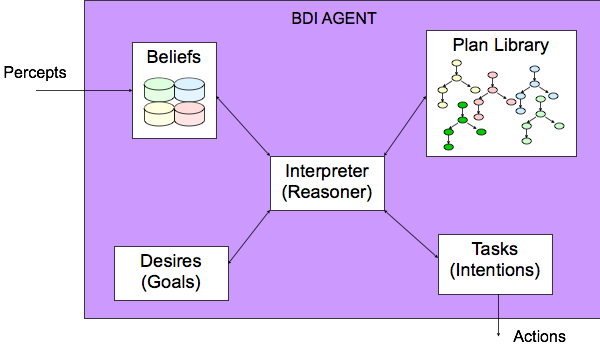
\includegraphics[width=0.7\textwidth]{reasoner} 
    \end{center} 
\end{frame} 

\begin{frame}{BDI Execution Concepts in JACK} 
    \begin{center}
        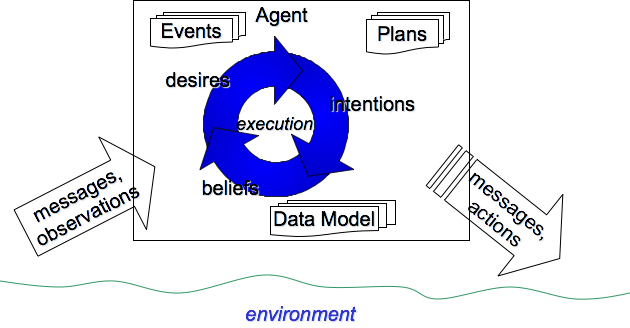
\includegraphics[width=0.8\textwidth]{execution} 
    \end{center} 
\end{frame} 

\begin{frame}{BDI Dynamics (1)}
    \begin{enumerate}
        \item An event occurs.
            \begin{itemize} 
                \item A goal is posted (internal).
                \item A change in the environment and hence a change in 
                      belief (external). 
            \end{itemize} 
        \item Agent reasoner searches through the plan library to
              find the set of plans which can handle this event
              (defined by the invocation condition).
        \item This may result in in 10 plans out of 500 which can
              handle the event. Out of these 10 plans, the agent
              reasoner then chooses only those which are 
              appropriate for this \textbf{context} -- that is, 
              the current situation. 
    \end{enumerate} 
\end{frame} 

\begin{frame}{BDI Dynamics (2)}
    \begin{enumerate}
        \setcounter{enumi}{4}
        \item This may result in 6 plans out of the 10 which are
              \textbf{applicable} in this context. 
        \item The agent then chooses one of the plans, puts it on the
              \textbf{intention stack}, and starts executing the plan
              steps in the plan.
        \item This executing plan is called an \textbf{intention} to 
              achieve the original \textbf{goal}. 
        \item If the plan fails, the agent will try on of the other
              applicable plans until one of them succeeds in 
              achieving the goal or all of them fail, in which case
              the goal will fail.
    \end{enumerate} 
\end{frame} 

\begin{frame}{BDI Dynamics Notes}
    \begin{itemize} 
        \item It is possible to determine which plan is chosen in the
              applicable plan set by using \textbf{meta-level reasoning}.
        \item Plans can wait until particular beliefs are satisfied.
        \item Plan steps can involve trying to achieve \textbf{sub-goals}.
        \item When trying to achieve a sub-goal, the existing plan
              is suspended and the new plan is put on top of the
              \textbf{intention stack}. 
    \end{itemize} 
\end{frame} 

\begin{frame}{Setting Up the JACK Environment} 
    \begin{alertblock}{These instructions were correct in 2003} 
        Needs Java 1.4.x, does not yet work with Java 1.5
        \begin{description}
            \item[Windows] 
                \texttt{set
                CLASSPATH=c:\textbackslash~aos\textbackslash~lib\textbackslash~jack.jar;.}
            \item[Bash] 
                \texttt{CLASSPATH=/aos/jack/lib/jack.jar:. export CLASSPATH} 
            \item[csh/tcsh]
                \texttt{setenv CLASSPATH=/usr/local/aos/jack/lib/jack.jar:. } 
        \end{description}
    \end{alertblock}
\end{frame} 

\begin{frame}{JACK File Types}
    \begin{description}
        \item[.jack] Any JACK object definition.
        \item[.agent] JACK agent definition.
        \item[.cap] JACK capability definition.
        \item[.plan] JACK plan definition.
        \item[.event] JACK event definition.
        \item[.bel] JACK beliefset definition.
        \item[.view] JACK view definition.
        \item[.java] Java class or interface definition. 
    \end{description}
\end{frame} 

\begin{frame}{Compiling JACK}
    The JACK Build is a two step process:
    \begin{enumerate}
        \item Generate Java code from the original 
              \texttt{.agent}, \texttt{.plan}, \texttt{.bel}
              \texttt{.event} etc. files.
        \item Compile the Java code
    \end{enumerate}
    \begin{block}{Building JACK code...}
        \begin{alltt}
            \$ java aos.main.JackBuild
        \end{alltt} 
    \end{block} 
    \begin{exampleblock}{Running is the same as Java programs...}
        \begin{alltt}
            \$ java Test
        \end{alltt} 
    \end{exampleblock} 
\end{frame} 

\begin{frame}{JACK Agent Language (JAL)} 
    The JACK Agent Language extends Java to support Agent Oriented programming:
    \begin{itemize}
        \item It defines new base classes, interfaces and methods. 
        \item It provides extensions to the Java syntax to support new 
              agent-oriented classes, definitions and statements. 
        \item It provides semantic extensions (runtime differences) 
              to support the execution model required by 
              an agent-oriented software system.
    \end{itemize} 
\end{frame} 

\begin{frame}{Class Level Constructs in JAL} 
    \begin{description}
        \item[Agent] Used to define the behaviour of an intelligent 
            software agent. This includes capabilities an agent has, 
            what type of messages and events it responds to and which plans it 
            will use to achieve its goals. 
        \item[Capability] Allows the functional components that make up an 
            agent to be aggregated and reused. A capability can be made up of 
            plans, events, beliefsets and other capabilities that together 
            serve to give an agent certain abilities. 
        \item[BeliefSet] The beliefset construct represents agent beliefs 
            using a generic relational model. 
        \item[View] The view construct allows general purpose queries to 
            be made about an underlying data model. 
            The data model may be implemented using multiple beliefsets 
            or arbitrary Java data structures. 
        \item[Event]The event construct describes an occurrence in 
            response to which the agent must take action. 
        \item[Plan] An agent's plans are analogous to functions. 
            They are the instructions the agent follows to try to 
            achieve its goals and handle its designated events. 
    \end{description} 
\end{frame} 

\begin{frame}{Example Agent Plan} 
    \showcode{robotplan.java} 
\end{frame} 

\begin{frame}{Agent Declarations -- \texttt{.agent}} 
    \begin{itemize}
        \item \emph{BeliefSets} and \emph{Views} which the agent can use and refer to. 
        \item \emph{Events} (both internal and external) that the 
               agent is prepared to handle. 
        \item \emph{Plans} that the agent can execute. 
        \item \emph{Events} the agent can post \textbf{internally} 
               (to be handled by other plans). 
        \item \emph{Events} the agent can send \textbf{externally} to other agents. 
    \end{itemize}
\end{frame} 

\begin{frame}{Example Pilot Agent \texttt{Pilot.agent}}
    \showcode{pilotagent.java} 
\end{frame} 

\begin{frame}{Events (\texttt{.event)} }
    \begin{itemize}
        \item Two broad categories of events
            \begin{enumerate}
                \item Normal events
                \item BDI events
            \end{enumerate} 

        \item The key difference between normal events and 
              BDI events is how an agent selects plans for execution.

        \item With normal events, the agent selects the first 
              applicable plan instance for a given event and executes 
              that plan instance only.


        \item The handling of BDI events is more complex and powerful. 
              An agent can assemble a plan set for a given event, 
              apply sophisticated heuristics for plan choice and 
              act intelligently on plan failure. 
    \end{itemize} 
\end{frame} 

\begin{frame}{Event Types in JACK} 
    \begin{itemize}
        \item Event
        \item MessageEvent
        \item BDIFactEvent
        \item BDIMessageEvent
        \item BDIGoalEvent
        \item InferenceGoalEvent
        \item PlanChoice
    \end{itemize} 
\end{frame} 

\begin{frame}{Example Event -- \texttt{TakeOffClearance.event}}
    \showcode{takeoffevent.java} 
\end{frame} 

\begin{frame}{Plans (.plans)} 
    \begin{itemize}
        \item The \texttt{Plan} class describes a sequence of actions that an 
              agent can take when an event occurs. 
        \item Whenever an event is posted and an agent adopts a 
              task to handle it, the first thing the agent does is 
              try to find a plan to handle the event.
        \item Plans can be thought of as pages from a procedures manual. 
              They describe, in explicit detail, exactly what an agent 
              should do when a given event occurs. 
        \item Each plan is capable of handling a single event. 
        \item When an instance of a given event arises, 
              the agent may execute one of the plans that 
              declare they handle this event. 
    \end{itemize} 
\end{frame} 

\begin{frame}{Discriminating Between Plans} 
    \begin{itemize}
        \item An agent may further discriminate between plans 
              that declare they handle an event by determining 
              whether a plan is relevant. 
        \item It does this by executing the \texttt{relevant()} method of each plan. 
        \item Once the relevant plan(s) have been identified, 
              the agent determines which of these are applicable. 
              It does this by executing the plans' \texttt{context()} method. 
          \item The context method is a JACK Agent Language logical \textbf{expression} 
              that can bind the values of the plan's logical members. 
        \item For every possible set of bindings, a separate applicable instance 
              of the plan is generated.
        \item When the agent has found all applicable instances of 
              each relevant plan, it selects one of these to execute.
    \end{itemize}
\end{frame}

\begin{frame}{Example Plan -- \texttt{TakeOff.plan}}
    \showcode{takeoffplan.java} 
\end{frame}

\begin{frame}{Reasoning Method Statements} 
    \begin{itemize}
        \item \texttt{@wait\_for(parameters)} 
        \item \texttt{ @action(parameters) <body> }
        \item \texttt{ @maintain(parameters) } 
        \item \texttt{ @post(parameters) }
        \item \texttt{ @reply(parameters) }
        \item \texttt{ @send(parameters) }
        \item \texttt{ @subtask(parameters) }
        \item \texttt{ @sleep(parameters) }
        \item \texttt{ @achieve(parameters) } 
        \item \texttt{ @insist(parameters) } 
        \item \texttt{ @test(parameters) } 
        \item \texttt{ @determine(parameters) } 
        \item \texttt{ @parallel(parameters) <body> } 
    \end{itemize}
\end{frame} 

\begin{frame}{Beliefset Declarations -- \texttt{.bel}}
    \begin{itemize}
        \item Beliefsets are used in JACK to maintain an agent's 
              beliefs about the world.
        \item An agent's beliefset can be stored as either an 
              OpenWorld or a ClosedWorld class. 
        \item The beliefset represents these beliefs in a first order, 
              tuple-based relational model 
    \end{itemize} 
    \begin{block}{Closed World Beliefs}
        True or False
    \end{block} 
    \begin{block}{Open World Beliefs}
        True, False or Unknown
    \end{block} 
\end{frame} 

\begin{frame}{Example Beliefset -- \texttt{BookData.bel}}
    \showcode{bookbelief.java} 
\end{frame} 

\begin{frame}{Jack Capabilities}
    \begin{itemize}
        \item A way to group related events, plans, beliefs, views etc.
        \item A way to make modular agent code.
        \item Groups related agent abilities together.
        \item Elements can belong to more than one capability.
        \item Like an ‘index’ of elements
            \begin{itemize}
                \item not a partitioning
                \item same element mentioned in many capabilities
            \end{itemize} 
        \item Module of elements that together implement a function (ability)
        \item Allows posting event in one capability, handling in another
        \item Allows data being hosted by one capability, used by another
        \item May be enabled / disabled dynamically
            \begin{itemize}
                \item if disabled, then its plans are not applicable
                \item no effect on data
            \end{itemize} 
    \end{itemize} 
\end{frame} 

\begin{frame}{Resources}
    \begin{itemize}
        \item \url{http://www.agent-software.com/}
        \item
            \url{http://agent-software.com/products/jack/documentation\_and\_instructi/}
    \end{itemize}
\end{frame} 

\end{document}
